\todo[inline]{Need to rename Q-routing in graphs}
\begin{figure}[ht]
	\begin{minipage}{.49\textwidth}
		\centering
		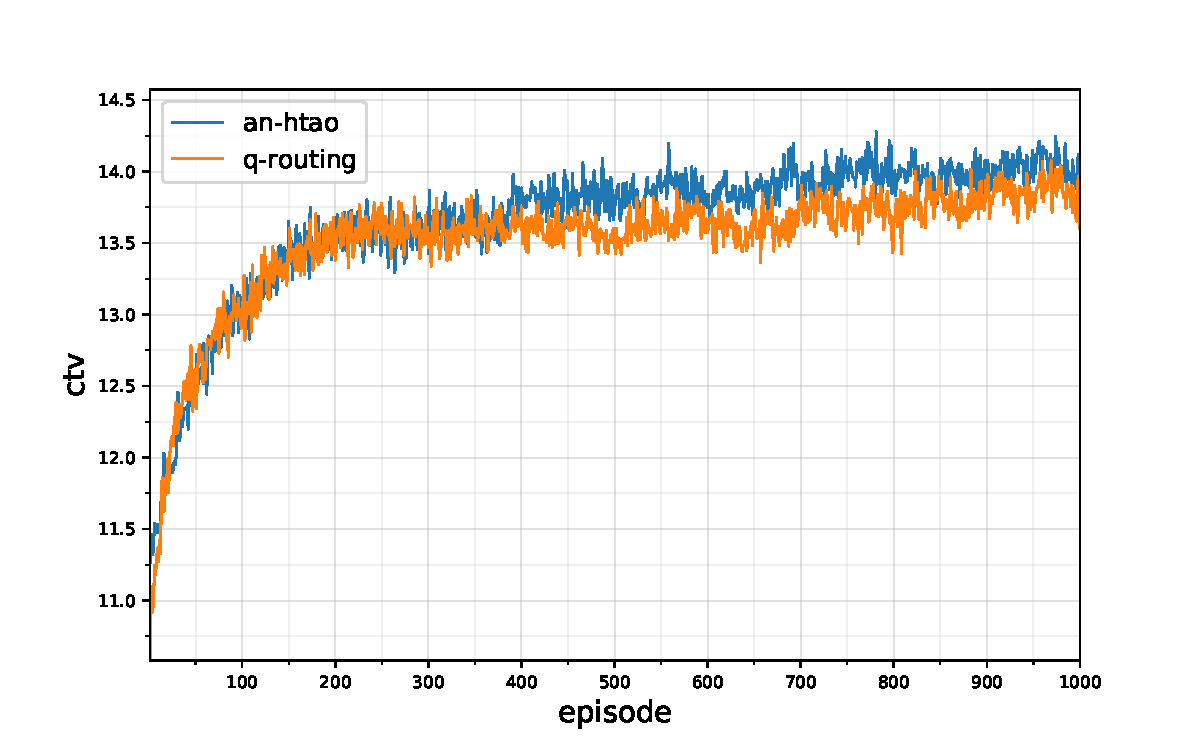
\includegraphics[width=1.0\linewidth,trim={25pt 0pt 50pt 0pt},clip]{520balanced_statistics-optimal-ctv}
		\captionsetup{labelfont=bf,singlelinecheck=on}
		\caption{Average system utility per-episode in the \newline \simulationSimple{}{} system.}
		\label{fig:simple_ctv}
	\end{minipage}
	\begin{minipage}{.49\textwidth}
		\centering
		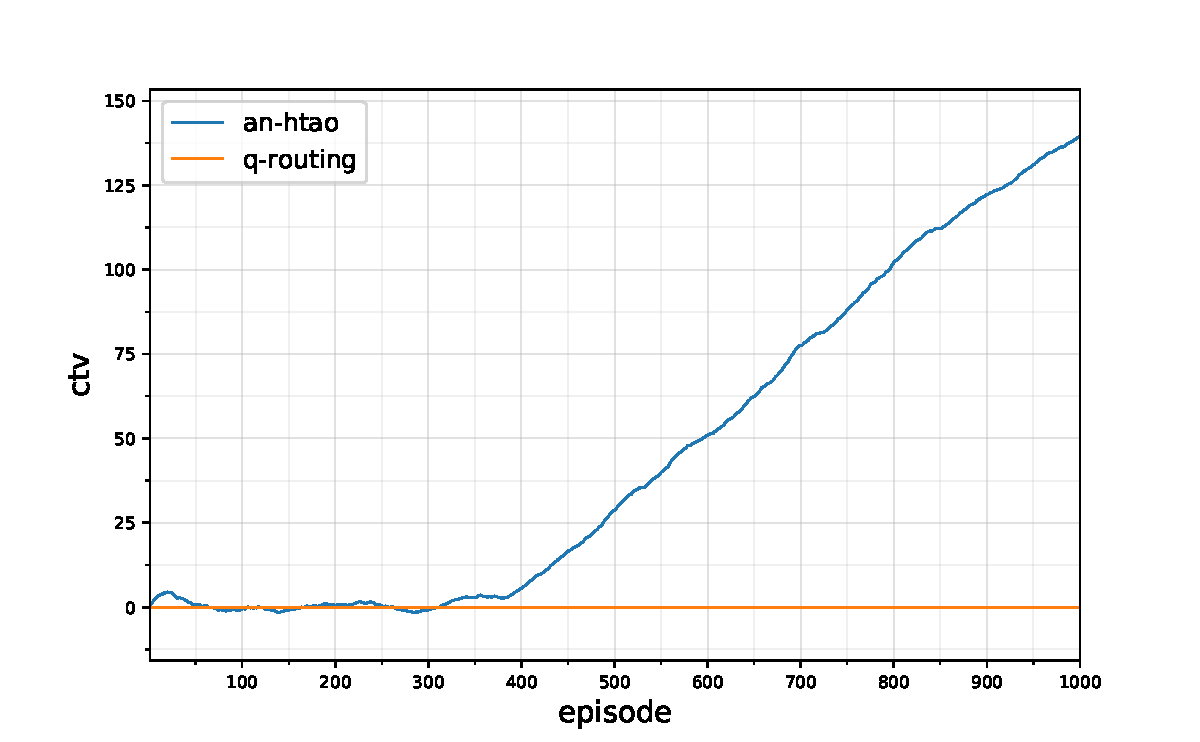
\includegraphics[width=1.0\linewidth,trim={25pt 0pt 50pt 0pt},clip]{520comparison_statistics-optimal-ctv-comparison-cumulative}
		\captionsetup{labelfont=bf,singlelinecheck=on}
		\caption{Cumulative system utility in the \simulationSimple{}{} system.}
		\label{fig:simple_cumulative_ctv}
	\end{minipage}\hfill% 
\end{figure}

\begin{figure}[ht]
	\begin{minipage}{.49\textwidth}
		\centering
		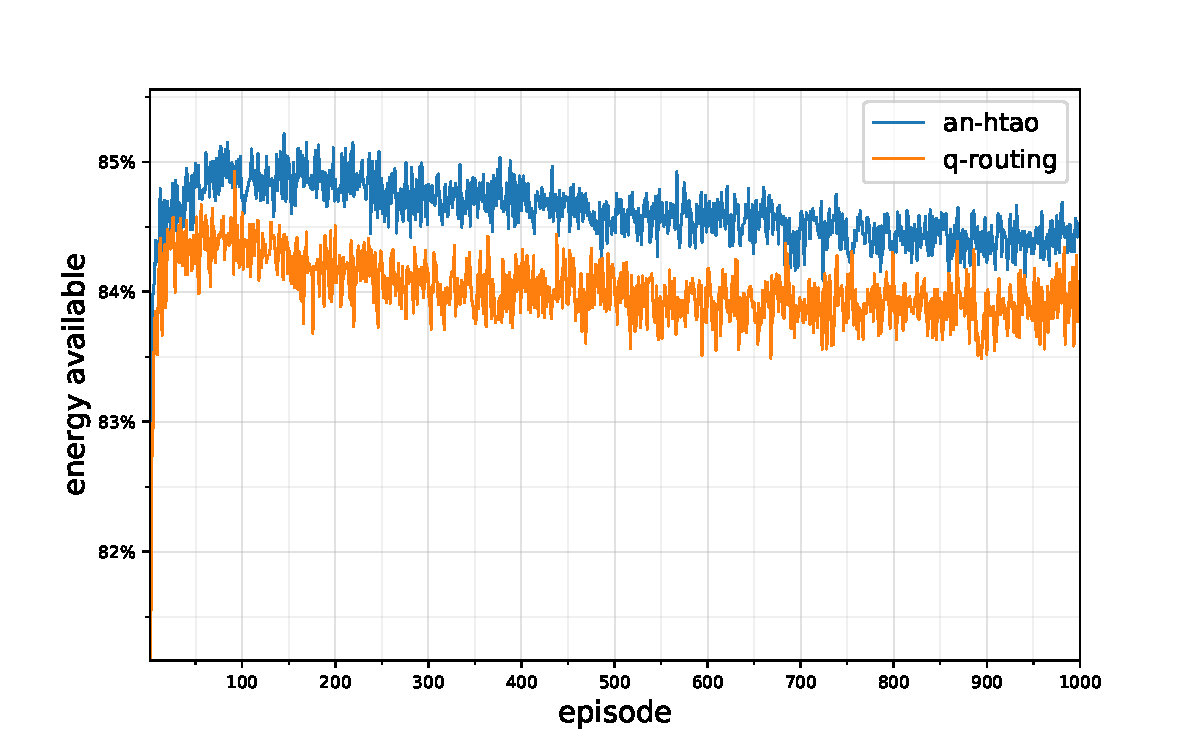
\includegraphics[width=1.0\linewidth,trim={25pt 0pt 50pt 0pt},clip]{520balanced_statistics-energy-available}
		\captionsetup{labelfont=bf,singlelinecheck=on}
		\caption{Percentage energy available  per-episode \newline in the \simulationSimple{}{} system.}
		\label{fig:simple_energy}
	\end{minipage}
	\begin{minipage}{.49\textwidth}
		\centering
		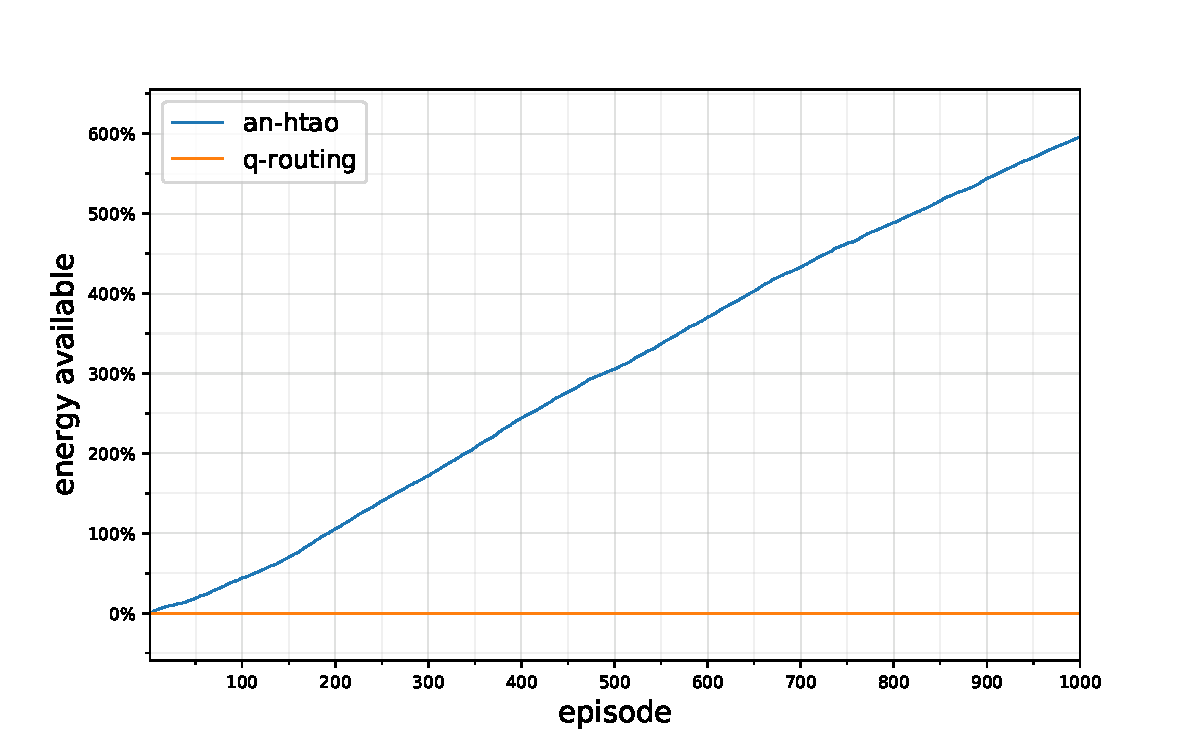
\includegraphics[width=1.0\linewidth,trim={25pt 0pt 50pt 0pt},clip]{520comparison_statistics-energy-available-baseline-comparison-cumulative}
		\captionsetup{labelfont=bf,singlelinecheck=on}
		\caption{Cumulative percentage energy available \newline in the \simulationSimple{}{} system.}
		\label{fig:simple_cumulative_energy}
	\end{minipage}\hfill% 
\end{figure}

\begin{figure}[ht]
	\begin{minipage}{.49\textwidth}
		\centering
		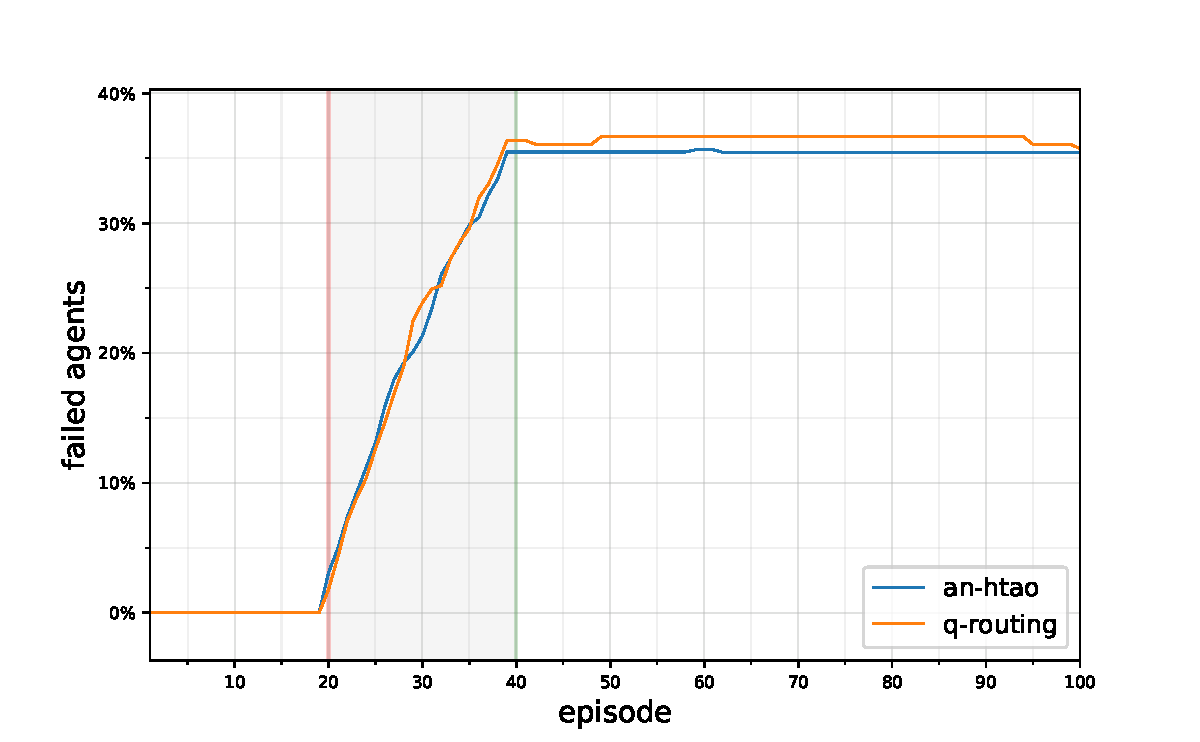
\includegraphics[width=1.0\linewidth,trim={25pt 0pt 50pt 0pt},clip]{7balanced_coverage-failed-agents}
		\captionsetup{labelfont=bf,singlelinecheck=on}
		\caption{Percentage of failed agents per-episode \newline in the \simulationNodeFailure{}{} system.}
		\label{fig:node_failure_failed_agents}
	\end{minipage}
	\begin{minipage}{.49\textwidth}
		\centering
		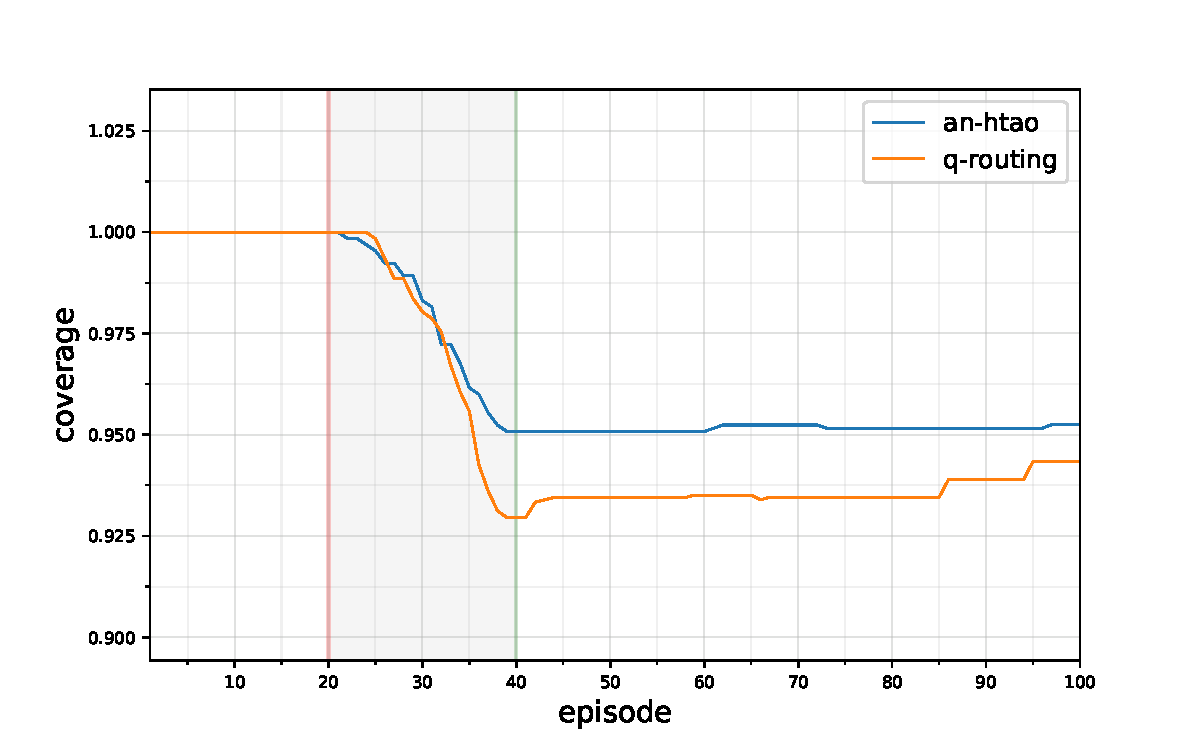
\includegraphics[width=1.0\linewidth,trim={25pt 0pt 50pt 0pt},clip]{7balanced_coverage-coverage}
		\captionsetup{labelfont=bf,singlelinecheck=on}
		\caption{System coverage in the \simulationNodeFailure{}{} \newline system.}
		\label{fig:node_failure_coverage}
	\end{minipage}\hfill% 
\end{figure}

\begin{figure}[ht]
	\begin{minipage}{.49\textwidth}
		\centering
		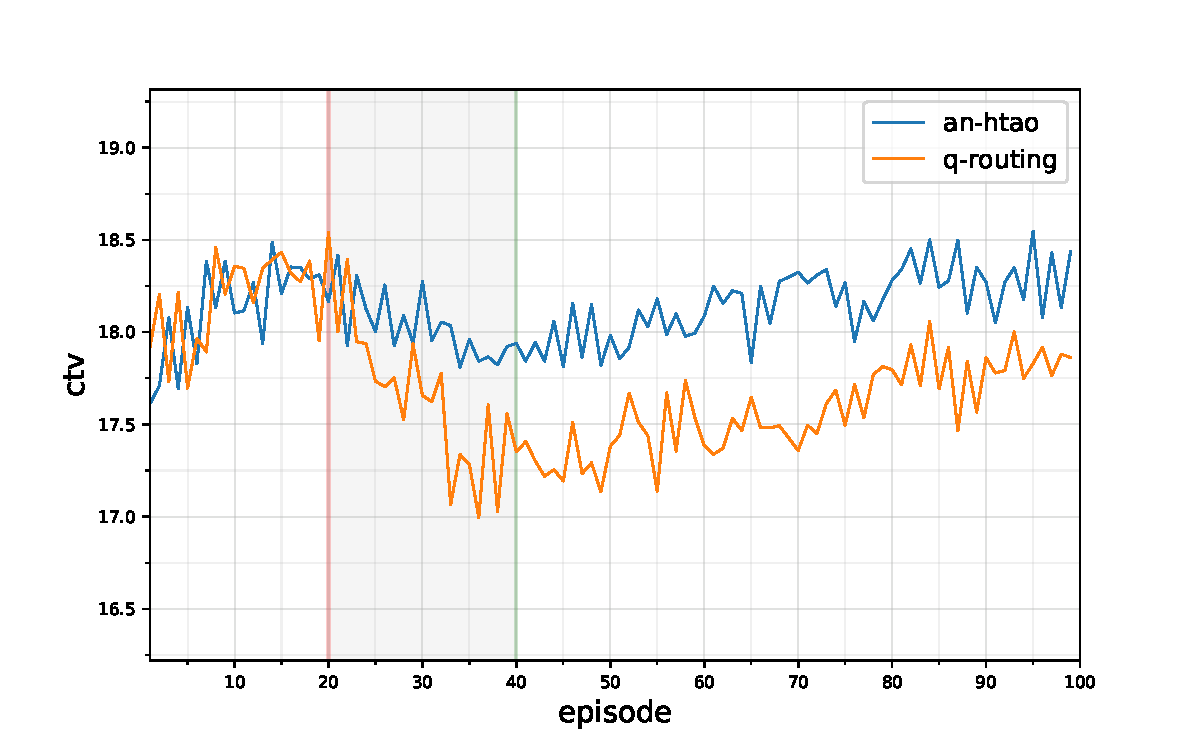
\includegraphics[width=1.0\linewidth,trim={25pt 0pt 50pt 0pt},clip]{7balanced_statistics-optimal-ctv}
		\captionsetup{labelfont=bf,singlelinecheck=on}
		\caption{System utility per-episode in the \newline \simulationNodeFailure{}{} system.}
		\label{fig:node_failure_ctv}
\end{minipage}
\begin{minipage}{.49\textwidth}
	\centering
	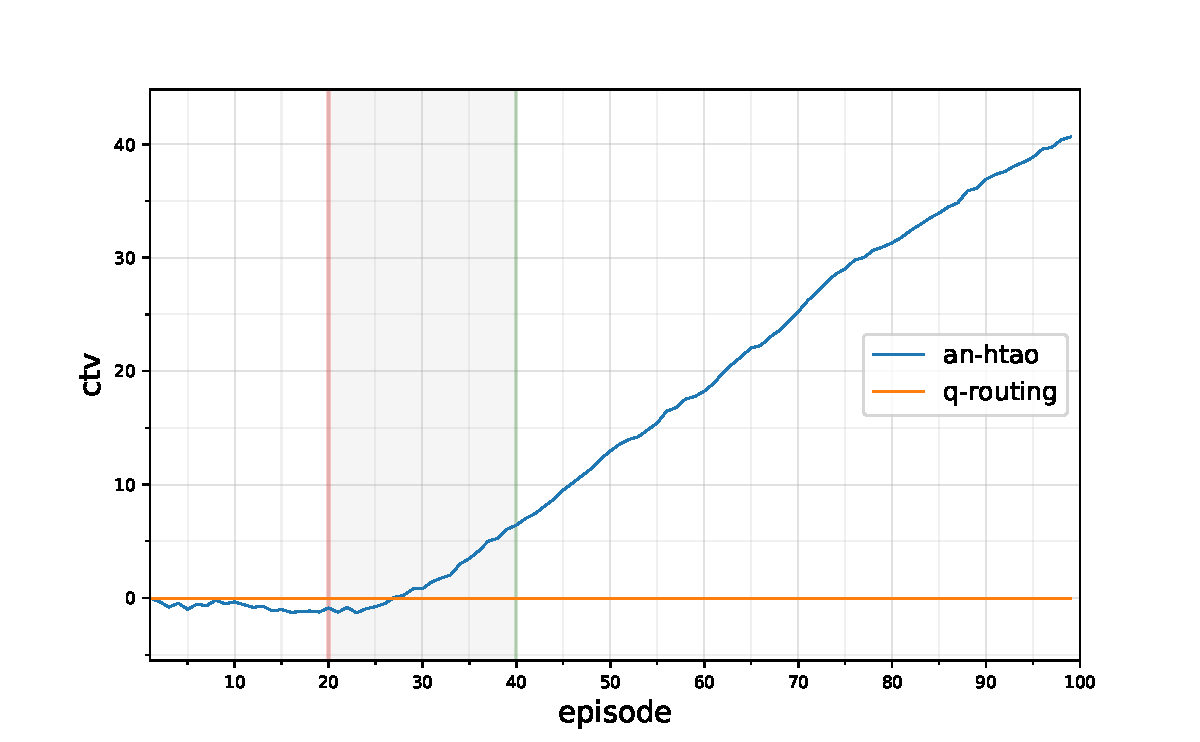
\includegraphics[width=1.0\linewidth,trim={25pt 0pt 50pt 0pt},clip]{7comparison_statistics-optimal-ctv-comparison-cumulative}
	\captionsetup{labelfont=bf,singlelinecheck=on}
		\caption{Cumulative system utility in the \simulationNodeFailure{}{}\newline system.}
		\label{fig:node_failure_cumulative_ctv}
\end{minipage}\hfill% 
\end{figure}

\begin{figure}[ht]
	\begin{minipage}{.49\textwidth}
		\centering
		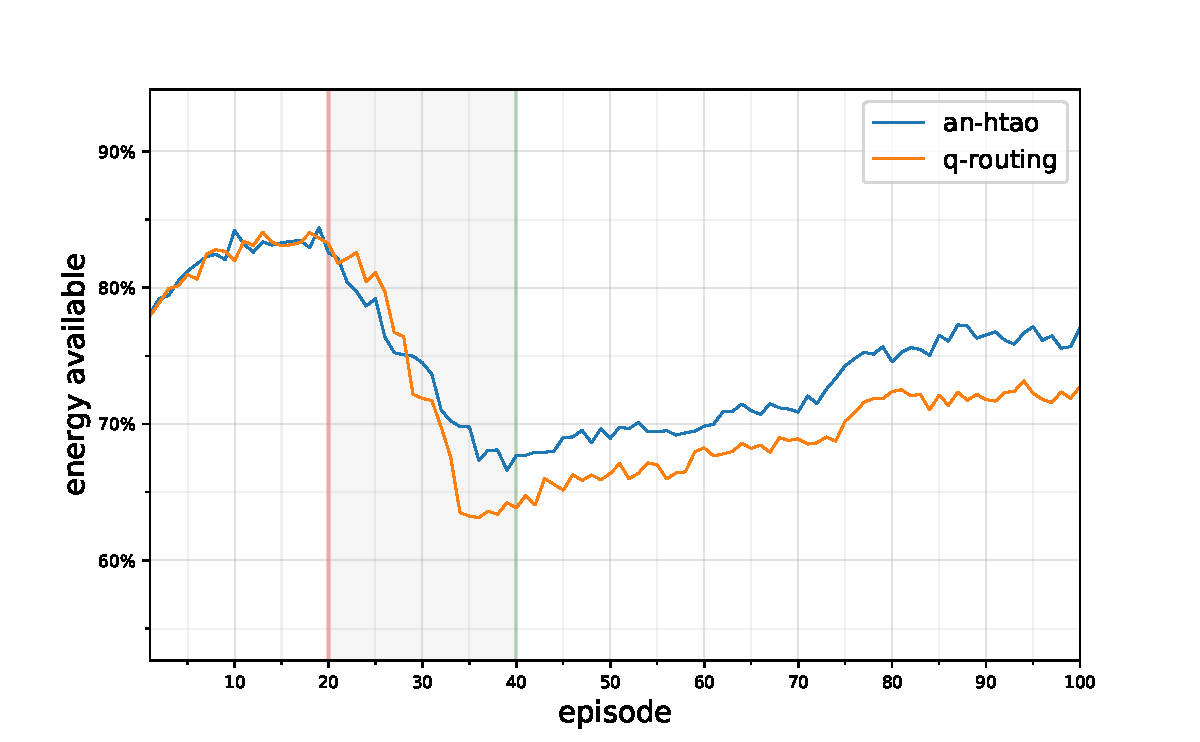
\includegraphics[width=1.0\linewidth,trim={25pt 0pt 50pt 0pt},clip]{7balanced_statistics-energy-available}
		\captionsetup{labelfont=bf,singlelinecheck=on}
		\caption{Percentage energy available per-episode \newline in the \simulationNodeFailure{}{} system.}
		\label{fig:node_failure_energy}
	\end{minipage}
	\begin{minipage}{.49\textwidth}
		\centering
		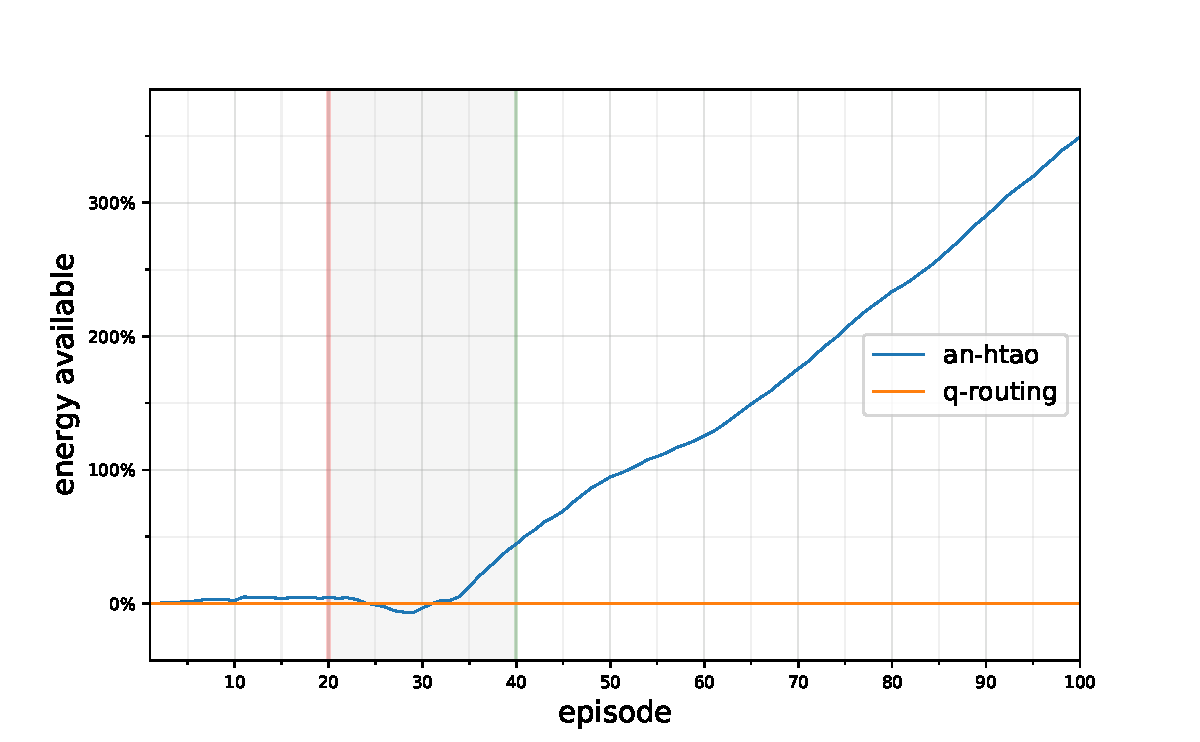
\includegraphics[width=1.0\linewidth,trim={25pt 0pt 50pt 0pt},clip]{7comparison_statistics-energy-available-baseline-comparison-cumulative}
		\captionsetup{labelfont=bf,singlelinecheck=on}
		\caption{Cumulative percentage energy available \newline in the \simulationNodeFailure{}{} system.}
		\label{fig:node_failure_cumulative_energy}
	\end{minipage}\hfill% 
\end{figure}

\begin{figure}[ht]
	\begin{minipage}{.49\textwidth}
		\centering
		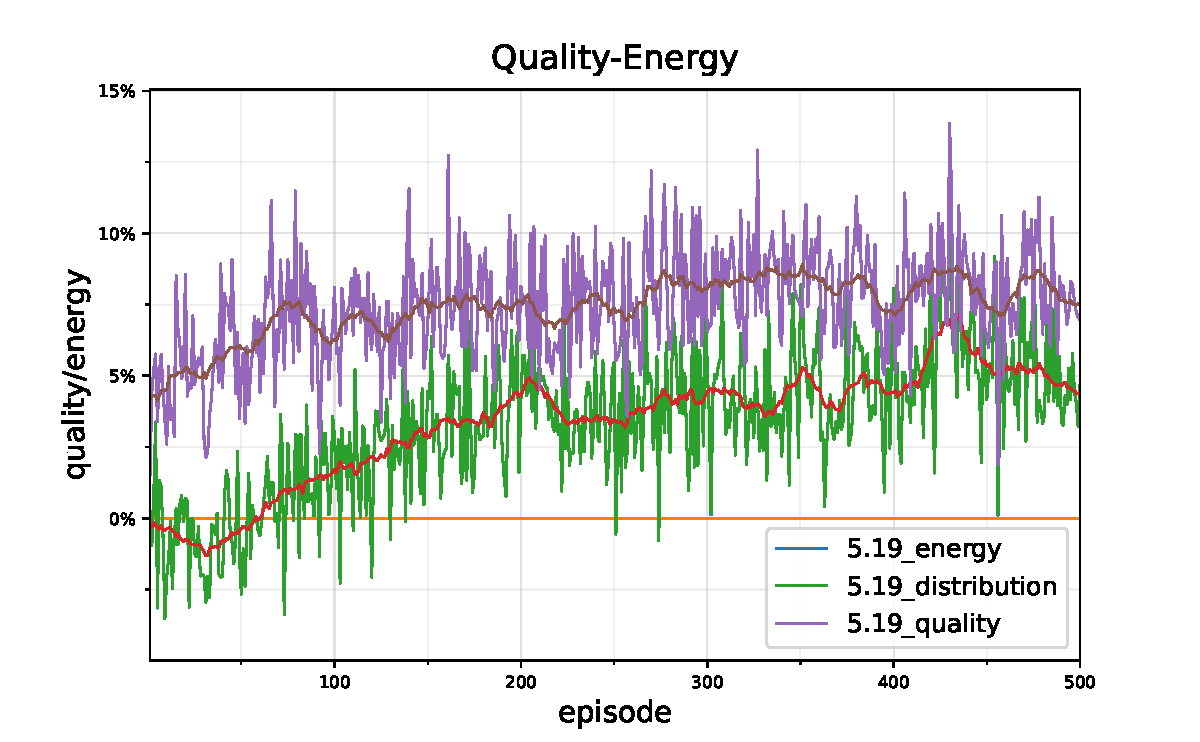
\includegraphics[width=1.0\linewidth,trim={25pt 0pt 50pt 0pt},clip]{5.19_ctv-quality-energy-baseline-comparison}
		\caption{Task quality to energy available ratio   with \newline \algorithmEnergy{}{} as the baseline in the \simulationExtended{}{} system}
		\label{fig:extended_quality_energy}
	\end{minipage}\hfill% 
	\begin{minipage}{.49\textwidth}
	\centering
	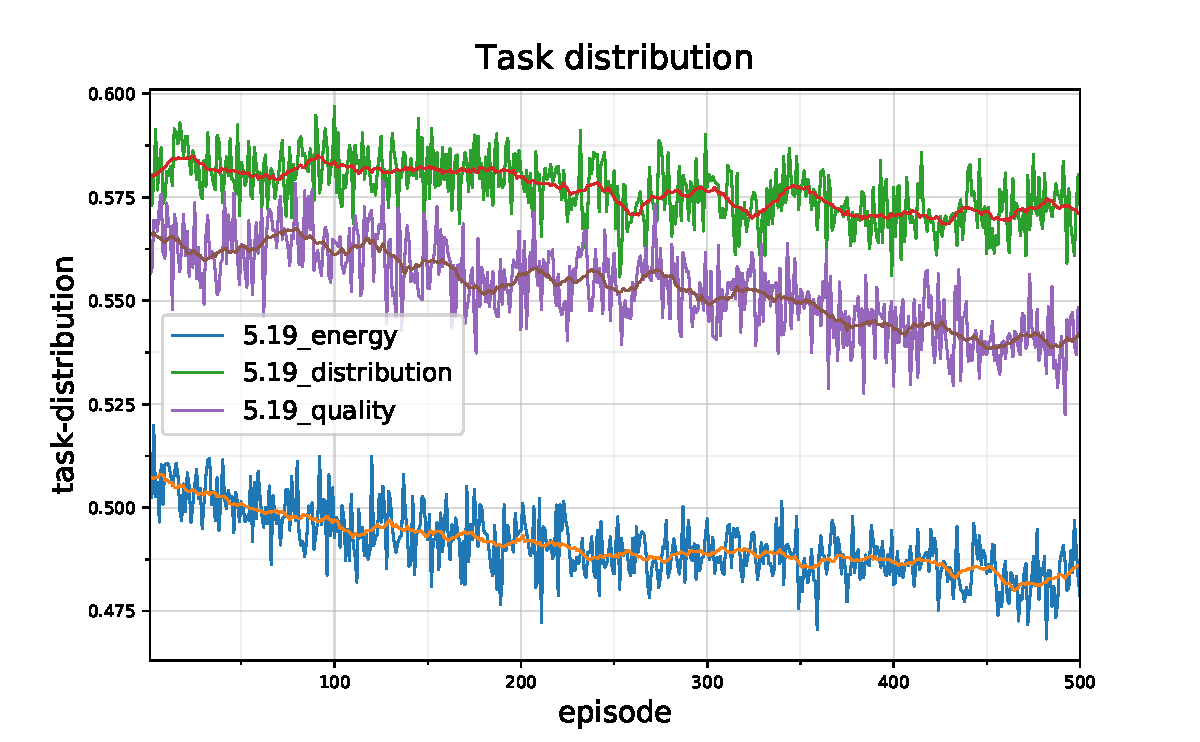
\includegraphics[width=1.0\linewidth,trim={25pt 0pt 50pt 0pt},clip]{5.19_ctv-task-distribution-comparison}
	\caption{The variance of unique sensor agents completing \newline atomic tasks  in the \simulationExtended{}{} system.}
		\label{fig:extended_task_distribution}
\end{minipage}
\end{figure}

\begin{figure}[ht]
	\begin{minipage}{.49\textwidth}
		\centering
		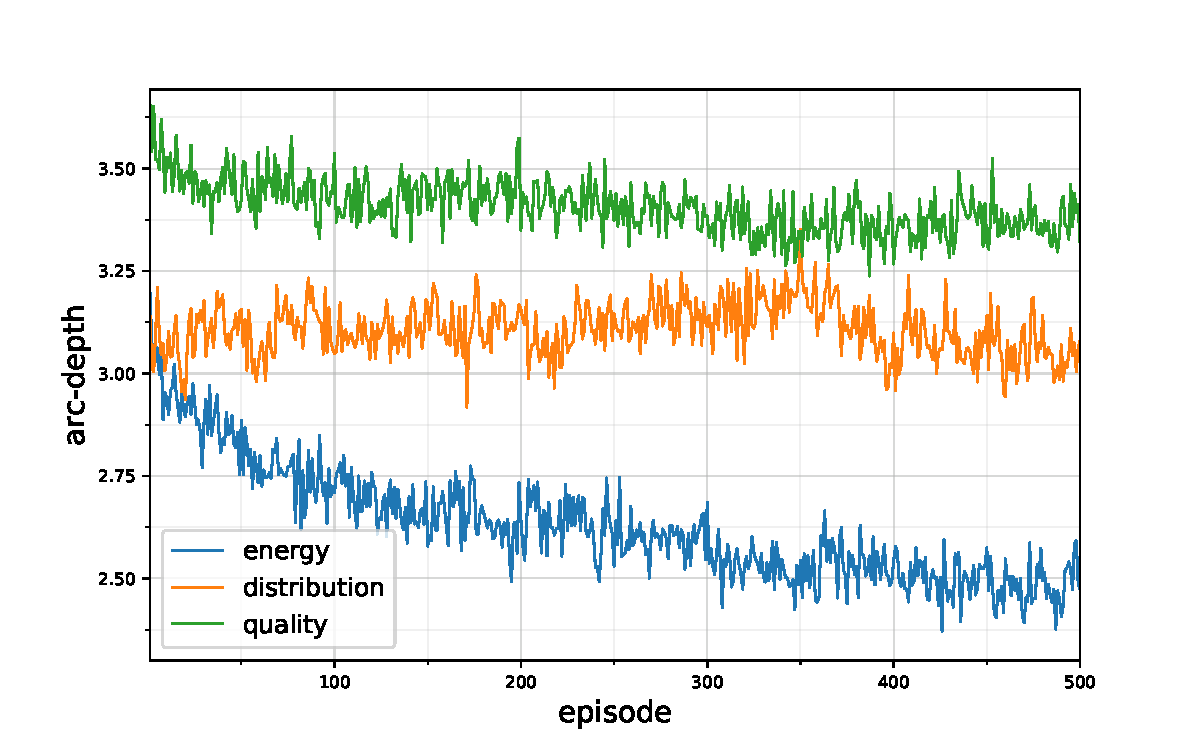
\includegraphics[width=1.0\linewidth,trim={25pt 0pt 50pt 0pt},clip]{5.19_ctv-arc-depth-comparison}
		\caption{Comparison of task-path depths  in the \simulationExtended{}{} system.}
		\label{fig:extended_arc_depth}
	\end{minipage}\hfill% 
\begin{minipage}{.49\textwidth}
\end{minipage}
\end{figure}

\subsection{Optimisation of utility, energy availability, and the  impact of agent loss on coverage}
In the \simulationSimple{}{} system, the \acronymWSNOptimisation{}{} algorithm optimised the system utility by \resultsSimpleCTVBalancedDiff{}{} over $1000$ episodes, compared to \resultsSimpleCTVQRoutingDiff{}{} for the \algorithmBaseline{}{} algorithm (Figures \ref{fig:simple_ctv} and \ref{fig:simple_energy}). Energy availability also increased by \resultsSimpleEnergyBalancedDiff{}{} for \algorithmBalanced{}{} algorithm and \resultsSimpleEnergyQRoutingDiff{}{} for \algorithmBaseline{}{}. Over the lifetime of the system the \algorithmBalanced{}{} algorithm accumulated \resultsSimpleCumulativeCTVComparison{}{} more utility than \algorithmBaseline{}{} and \resultsSimpleCumulativeEnergyComparison{}{} more energy availability (Figures \ref{fig:simple_cumulative_ctv} and \ref{fig:simple_cumulative_energy} ).

From Figure \ref{fig:node_failure_failed_agents} we can see that, in the \simulationNodeFailure{}{} system, as we gradually simulate the failure of agents from episode $20$ to $40$,  \resultsNodeFailureFailedAgentsBalancedDiff{}{} of them become unavailable. The coverage  of tasks using the \algorithmBalanced{}{} algorithm falls by \resultsNodeFailureCoverageBalancedDiff{}{} during this period, a $5.5\%$ improvement on  the \resultsNodeFailureCoverageQRoutingDiff{}{} drop of the \algorithmBaseline{}{} algorithm. The ability of the \algorithmBalanced{}{} algorithm to absorb agent failure better than the \algorithmBaseline{}{} algorithm is also seen in both the impact on system utility, \resultsNodeFailureCTVBalancedImpactDiff{}{} as compared to \resultsNodeFailureCTVQRoutingImpactDiff{}{}, and for the energy available, \resultsNodeFailureCTVBalancedImpactDiff{}{} compared to \resultsNodeFailureCTVQRoutingImpactDiff{}{}.


\subsection{Algorithm adaptability and system behaviour}

We now look at the \simulationExtended{}{} system in detail to examine how the algorithm vary the balance  of optimisation over the CTV components, allowing multiple-objectives to be targeted. Figure 	\ref{fig:extended_quality_energy} shows the task quality to energy availability ratio. 
As quality is preferentially optimised for over energy availability, values range higher. The \algorithmQuality{}{} algorithm, with its higher $\gamma$ value, optimises for task values by \resultsQEQualityEnd{}{} over the \algorithmEnergy{}{} algorithm, and the \algorithmDistribution{}{} algorithm by \resultsQEDistDiff{}{}. 

In Figure \ref{fig:extended_task_distribution} we see how completed atomic tasks are distributed in the system. This is measured by the variance in the sensor agents that complete atomic tasks, where lower values indicate some sensor agents are completing multiple tasks. In the \algorithmDistribution{}{} algorithm, values remain relatively steady throughout the system lifetime at \resultsTaskDistDistStart{}{} to \resultsTaskDistDistEnd{}{}, dropping only \resultsTaskDistDistPercent{}{}. The \algorithmQuality{}{} algorithm starts slightly lower than this at \resultsTaskDistQualityStart{}{} and falls \resultsTaskDistQualityPercent{}{} to \resultsTaskDistQualityEnd{}{}. Notably the \algorithmEnergy{}{} algorithm starts and remains at a significantly lower distribution than both these algorithms at \resultsTaskDistEnergyEnd{}{}, dropping \resultsTaskDistEnergydPercent{}{}. Figure
\ref{fig:extended_arc_depth} shows the related effect on task-path depths for each algorithm. The \algorithmQuality{}{} and \algorithmDistribution{}{} algorithms have relatively stable task-path depths at \resultsArcDepthQualityEnd{}{} and \resultsArcDepthDistEnd{}{} respectively. The average task-path depth of the \algorithmEnergy{}{} algorithm however drops from \resultsArcDepthEnergyStart{}{} to  \resultsArcDepthEnergyEnd{}{} over the systems' lifetime, a \resultsArcDepthEnergyPercent{}{} decrease.

\begin{figure}
	\centering
	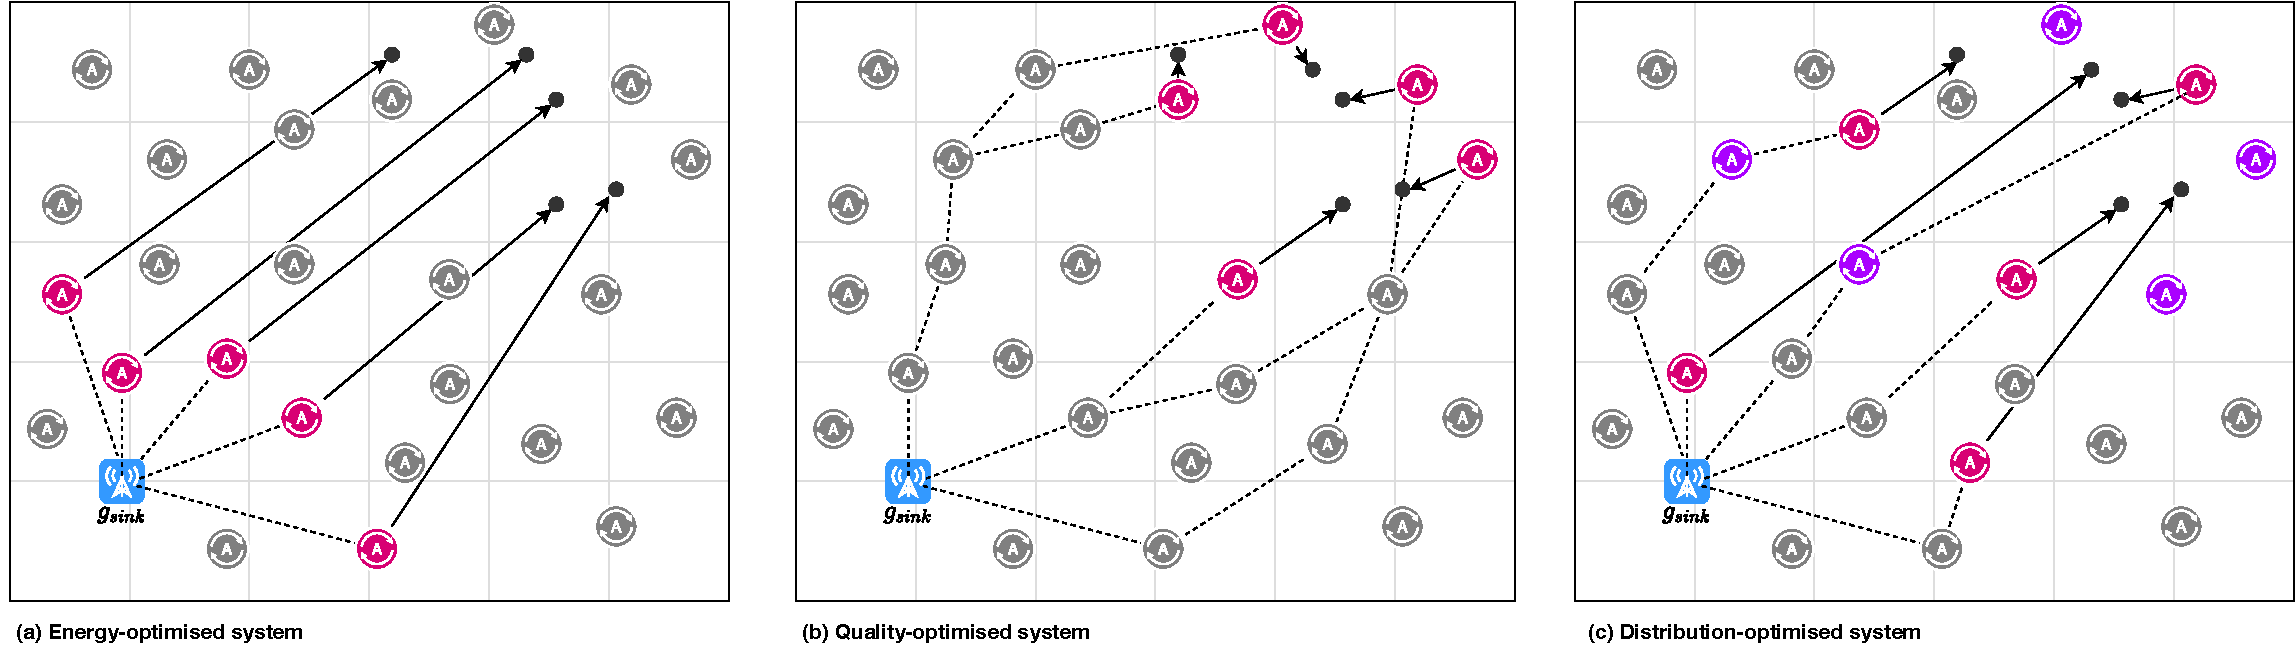
\includegraphics[width=1.0\linewidth]{result-types}
	\caption{Three sample task-path patterns in the \simulationExtended{}{} system. In the \algorithmEnergy{}{}-optimised configuration (a), the sensing agents are near the sync agent. Energy use is minimised but the measurements task-values are low. In the \algorithmQuality{}{}-optimised configuration (b) the sensing agents are close to the demand points, maximising the task-values, however there is an increase in energy usage as they are more distant from the sink, with increased task-path depth. In the \algorithmDistribution{}{}-optimised configuration (c), sensing agents are a mix of close and further away from the demand points, with an the agents participating in the task-paths changing with different measurements}
	\label{fig:result-types}
\end{figure} 

Relating these results to the systems in Figure \ref{fig:result-types}, the \algorithmEnergy{}{} algorithm is close to configuration in Figure \ref{fig:result-types}$(a)$, where energy consumption is reduced by using shorter task-paths and so, the amount of energy used by agents in the system to broadcast task re-allocations. The cost of this is that the tasks are completed to a lower quality. In Figure \ref{fig:result-types}$(c)$, task-path depths are large so that tasks can be completed by agents close to their demand points, increasing task quality as well as consumption, as seen in the results for the \algorithmQuality{}{} algorithm. The configuration in Figure \ref{fig:result-types}$(b)$ explains the results seen with the \algorithmDistribution{}{} algorithm, where tasks are completed by an increased number of different agents with different task-path depths and task qualities, giving a greater distribution of task completions and energy usage, but with more energy consumption overall than the \algorithmEnergy{}{} algorithm, and less task-quality than the \algorithmQuality{}{} algorithm.

As seen in both the \simulationSimple{}{}  and \simulationNodeFailure{}{} system configurations, utility and energy availability are both optimised by the algorithm, and improve on the comparison \algorithmBaseline{}{} algorithm. Through the \simulationNodeFailure{}{} results we see that this performance extends to realistic real-world systems with instability, adapting task routing to maintain coverage as agents are lost.  Additionally, the results of the \acronymWSNOptimisation{}{} energy, quality, and distribution-optimised algorithms in the \simulationExtended{}{} system show that we can adapt the balance of the CTV components through varying values of $\alpha$, $\beta$, and $\gamma$, to achieve an adaptive multi-objective optimisation of the system. These results show that the algorithm achieves the main goals for applications in WSN as laid out in Section \ref{section:problem:statement}.

With a CTV balance optimised solely to minimise energy consumption, i.e. $(\alpha=1,\beta=0,\gamma=0)$, the \acronymWSNOptimisation{}{} algorithm behaves similarly to energy-aware algorithms applied to WSN. In this configuration comparisons can be made with algorithms such as PEGASIS \citep{Lindsey2002}, or more closely to Q-routing algorithms like Q-probabilistic routing \citep{Arroyo-Valles2007}. However, the task allocation and resource optimisation component of the \acronymWSNOptimisation{}{} algorithm is not accounted for in these implementations so provides only a comparison for the energy and route adaptation properties. 
